% asset_id: AS1QuadraticsTikZ-003
% source: Quadratics modelling transcript evidence, including projectile-style height models
% related_section: Core Theory Part I – Modelling with Quadratics
% purpose: Projectile-style quadratic diagram showing starting height, maximum and ground intersection.
\documentclass[tikz,border=8pt]{standalone}
\usetikzlibrary{arrows.meta,calc}
\begin{document}
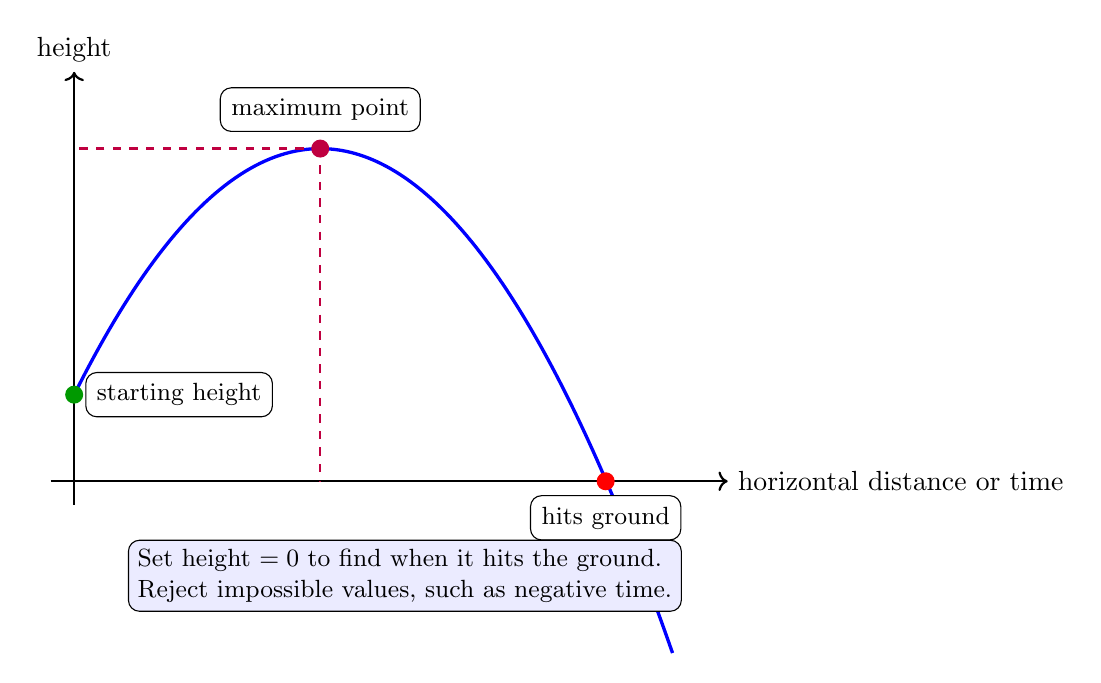
\begin{tikzpicture}[axis/.style={->, thick},curve/.style={very thick, blue},guide/.style={dashed, thick},point/.style={circle, fill=red, inner sep=2.3pt},labelbox/.style={draw, rounded corners, fill=white, inner sep=4pt, font=\small}]
\draw[axis] (-0.3,0) -- (8.3,0) node[right] {horizontal distance or time};
\draw[axis] (0,-0.3) -- (0,5.2) node[above] {height};
\draw[curve, domain=0:7.6, samples=120] plot (\x,{1.1 + 2.0*\x - 0.32*\x*\x});
\node[point, fill=green!60!black] at (0,1.1) {}; \node[labelbox, right=4pt] at (0,1.1) {starting height};
\coordinate (M) at (3.125,4.225); \node[point, fill=purple] at (M) {}; \node[labelbox, above=6pt] at (M) {maximum point};
\draw[guide, purple] (M) -- (3.125,0); \draw[guide, purple] (M) -- (0,4.225);
\coordinate (G) at (6.75,0); \node[point] at (G) {}; \node[labelbox, below=5pt] at (G) {hits ground};
\node[draw, rounded corners, fill=blue!8, align=left, font=\small] at (4.2,-1.2) {Set height $=0$ to find when it hits the ground.\\Reject impossible values, such as negative time.};
\end{tikzpicture}
\end{document}
